\section{Contexte biologique et naissance du modèle}


%Diapo 1
\begin{frame}
\frametitle{Contexte biologique et naissance du modèle}
\framesubtitle{Polarisation, dépolarisation et canaux ioniques}

\begin{columns}
\column{0.5\textwidth}
\begin{small}
\begin{itemize}
  \item \textbf{Au repos} : l'intérieur de la cellule est négatif ($\approx -70$ mV) par rapport à l'extérieur : c'est la \alert{polarisation}.
  \item Maintien par la pompe Na$^+$/K$^+$ et des canaux de fuite.
  \item \textbf{Dépolarisation} : ouverture de canaux Na$^+$ voltage‑dépendants $\rightarrow$ entrée de Na$^+$ $\rightarrow$ le potentiel devient positif.
  \item \textbf{Repolarisation} : inactivation des canaux Na$^+$, ouverture de canaux K$^+$ $\rightarrow$ sortie de K$^+$ $\rightarrow$ retour au repos.
\end{itemize}
\end{small}
\column{0.5\textwidth}
\begin{figure}[t]
    \centering
    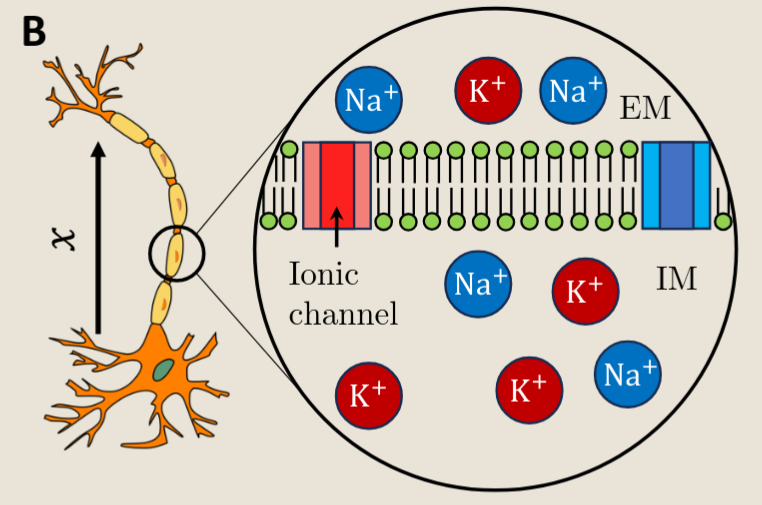
\includegraphics[width=\linewidth]{Figures/canaux_ioniques.png}
    \caption{Canaux ioniques}
    %\source{Six decades of the FitzHugh-Nagumo model: A guide through its spatio-
%temporal dynamics and influence across disciplines}
\end{figure}
\end{columns}
\end{frame}

%Diapo 2
\begin{frame}
\frametitle{Contexte biologique et naissance du modèle}
\framesubtitle{L'excitabilité des cellules cardiaques}
\begin{columns}
\column{0.6\textwidth}
\begin{itemize}
  \item Les cellules du muscle cardiaque (cardiomyocytes) sont \alert{excitables}.
  \item Un stimulus suffisant déclenche un \textbf{potentiel d'action} : 
    dépolarisation rapide suivie d'une repolarisation.
  \item Ce signal électrique se propage de proche en proche et coordonne la contraction.
\end{itemize}
\column{0.4\textwidth}

\begin{figure}
    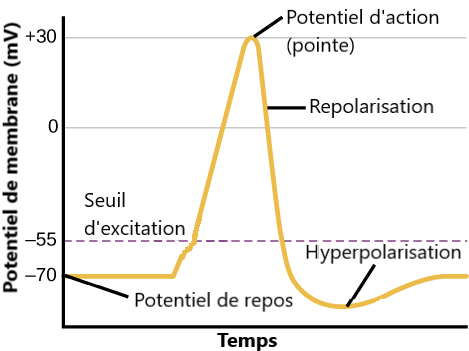
\includegraphics[width=\linewidth]{Figures/potentiel_action.png}
    \caption{Potentiel d'action} \label{Figure-1}
    %\source{ Image modifiée à partir de "How neurons communicate: Figure 3," par OpenStax College, Biology (CC BY 3.0).}
\end{figure}
\end{columns}
\end{frame}

%Diapo 3
\begin{frame}
\frametitle{Contexte biologique et naissance du modèle}
\framesubtitle{Modèle de Hodgkin-Huxley (1952) – Circuit équivalent}
\centering
\begin{figure}
  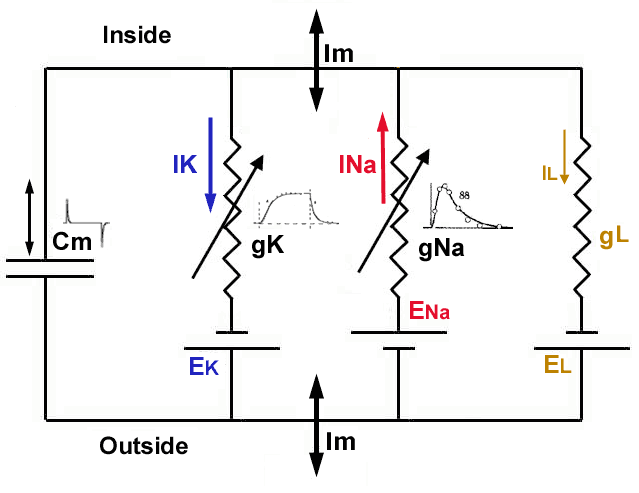
\includegraphics[scale = 0.35]{Figures/HH.png} 
  \caption{Circuit équivalent : 4 branches parallèles (Na\(^+\), K\(^+\), fuite, capacité).}
  %\source{University of Pennsylvania School of Arts and Sciences. (n.d.). Circuit diagram and related equation. SAS Lab Manuals.}
\vspace{0.3cm}
\end{figure}
\end{frame}



%Diapo 4
\begin{frame}
\frametitle{Contexte biologique et naissance du modèle}
\framesubtitle{Modèle de Hodgkin-Huxley (1952) – description mathématique}
%\column{0.6\textwidth}
\textbf{Équation de la membrane :}
\[
C_m\frac{dV}{dt} = -\underbrace{\bar{g}_{\text{Na}} m^3 h (V-E_{\text{Na}})}_{\text{courant Na\(^+\)}}
                 -\underbrace{\bar{g}_{\text{K}} n^4 (V-E_{\text{K}})}_{\text{courant K\(^+\)}}
                 -\underbrace{g_{\text{L}}(V-E_{\text{L}})}_{\text{fuite}}
                 + I_{\text{app}}
\]
\textbf{Équations des portes (gating) :}
\[
\frac{dm}{dt} = \alpha_m(V)(1-m) - \beta_m(V)m \quad \text{(activation Na\(^+\))}
\]
\[
\frac{dh}{dt} = \alpha_h(V)(1-h) - \beta_h(V)h \quad \text{(inactivation Na\(^+\))}
\]
\[
\frac{dn}{dt} = \alpha_n(V)(1-n) - \beta_n(V)n \quad \text{(activation K\(^+\))}
\]
\end{frame}


%Diapo 5
%\begin{frame}
%\frametitle{Contexte biologique et naissance du modèle}
%\framesubtitle{Difficultés du modèle Hodgkin‑Huxley}
%\begin{itemize}
%  \item \textbf{Système à 4 variables} : $V$, $m$, $h$, $n$ $\Rightarrow$ espace des phases de dimension 4.
%  \item \textbf{Non‑linéarités complexes} : les taux $\alpha(V)$, $\beta(V)$ et les produits de puissances ($m^3h$, $n^4$).
%  \item \textbf{Absence d’outils géométriques simples} :
%  \begin{itemize}
%    \item Pas de portrait de phase en 2D.
%    \item Pas d’isoclines visuellement exploitables.
%  \end{itemize}
%  \item \textbf{Impossible d’obtenir des formules analytiques} pour :
%  \begin{itemize}
%    \item le seuil d’excitation,
%    \item la fréquence des oscillations,
%    \item les conditions de bifurcation.
%  \end{itemize}
%  \item \textbf{Coût de simulation prohibitif} pour de grands réseaux :
%  \begin{itemize}
%    \item Un tissu cardiaque $\approx 10^6$ cellules $\times$ 4 EDOs $\Rightarrow$ millions d’équations.
%  \end{itemize}
%\end{itemize}
%\end{frame}

%Diapo 6
\begin{frame}
\frametitle{Contexte biologique et naissance du modèle}
\framesubtitle{La réduction de FitzHugh‑Nagumo (1961)}
\alert{\textbf{En exploitant les échelles de temps}}
\begin{itemize}
  \item Dans HH, la porte d’activation sodium $m$ est \textbf{très rapide} : $m \approx m_\infty(V)$ (instantanée).
  \item Les variables $h$ (inactivation Na$^+$) et $n$ (activation K$^+$) évoluent \textbf{lentement} et sont \textbf{corrélées}.
  \item On les remplace par une seule variable lente $w$ (récupération).
\end{itemize}

\alert{\textbf{Le modèle à 2 variables}}
\[
\begin{cases}
  \displaystyle \frac{dv}{dt} = v - \frac{v^3}{3} - w + I_{\text{app}} \\[8pt]
  \displaystyle \frac{dw}{dt} = \varepsilon (v + a - b w)
\end{cases}
\]
\begin{itemize}
  \item $v$ : variable rapide (potentiel de membrane).
  \item $w$ : variable lente (recouvrement).
  \item $\varepsilon \ll 1$ : petit paramètre garantissant la séparation d’échelles.
  \item $a$, $b$, $I_{\text{app}}$ : paramètres de contrôle du comportement.
\end{itemize}
\end{frame}